    
\documentclass[11pt]{article}
\usepackage{graphicx}
\graphicspath{ {./images/} }
\usepackage{times}
    \usepackage{fullpage}
    
    \title{Integrated Visual Field Remapping for Hemianopia}
    \author{ {Nik Harith Sharifuddin} - {2673209B }}

    \begin{document}
    
    \maketitle
    
    
     

\section{Status report}

\subsection{Proposal}\label{proposal}

\subsubsection{Aims}\label{aims}

The goal of this project is to design and develop a Virtual Reality (VR) application that enables the user to remap the visuals of that are displayed in the VR headset to 'fit' into the user's limited visual field. Moreover, the application will have the capability to take in data of a visual field test and automatically calculates and implement the remapping function based on it. The project also aims to integrate this remapping function module with the visual testing module made by another student.

By the end of this project, there will be a deployable application that would enable the functionalities above and would also integrate with the visual field testing module in a single platform.

\subsubsection{Motivation}\label{motivation}

Hemianopia is a condition usually caused by stroke where the visual field of the patient is limited to half of the whole region. This condition can affect either on one or both of the eyes and patients have reported difficulties carrying out their daily activities such as navigating, using mobile devices and reading.

In recent years, the advancement of Virtual Reality (VR) technology have introduced head-mountable devices (HMD) or simply called 'headsets' that offers capabilities such as live camera feed and eye tracking. These capabilities offers novel opportunities to provide an accessible solution for hemianopia patients to increase their visual field and aid with their daily activities. 



\subsection{Progress}\label{progress}


\begin{itemize}
% \tightlist
    \item   Language and platform chosen: project will be using Unity with C\# as its scripting language.
    \item   Standardization of Unity version has been decided at version 2022.3.40f with other student that is working for the visual testing module.
    \item   Initialised shared Gitlab repository for easy integration of the two modules.
    \item   Literature review conducted on hemianopia, possible recovery and the state-of-art of using VR in ophthalmology.
    \item   Entity-relation diagram  of the system designed.
    \item   Basic interface has been made to navigate into the two modules.
    \item   Previous version of the remapping module has been explored and tested.

\end{itemize}

\subsection{Problems and risks}\label{problems-and-risks}

\subsubsection{Problems}\label{problems}

\begin{itemize}

    \item   Complexity of the problem has delayed the formulation of design works for the system.
    \item   Multiple coinciding deadlines of coursework taken in Semester 1 resulted in reduced time contributing to the project - this is resolved by next semester as the critical courses have been taken.
    \item   Keys to access supervisor's office for dedicated PCs and VR headsets to work on has not yet been obtained.

\end{itemize}


\subsubsection{Risks}\label{risks}

\begin{itemize}
    \item   Not getting timely access to dedicated workstations in supervisor's office. \textbf{Mitigation:} Request the keys to the room as soon as possible
    \item   Uncertainty on choosing the evaluation methods to evaluate the success of the project. \textbf{Mitigation: } Review researched literature materials to gain insights how previous attempts were evaluated.


\end{itemize}

\subsection{Plan}\label{plan}

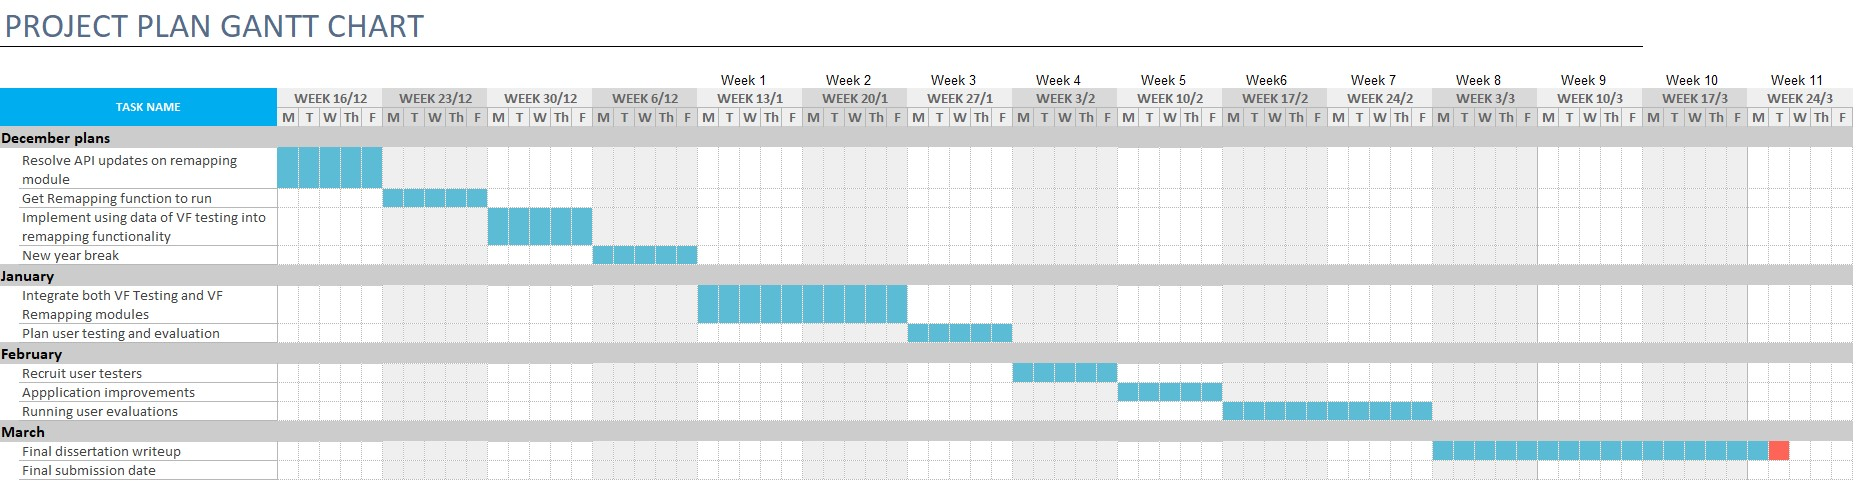
\includegraphics[width=\textwidth]{images/INP-full-ganttChart.jpg}

\subsubsection{December plans}
\begin{itemize}
    \item Week starting \textbf{16 December} - update APIs in previous implementations.
    \item Week starting \textbf{23 December} - Test remapping function to run nicely. Think about how to conduct user testing.
    \item Week starting \textbf{30 Dec} - Integrating data of VF testing into the remapping module and performing the remap based on the data.
    
\end{itemize}

\subsubsection{Semester 2}

\begin{itemize}
    \item   \textbf{Week 1-2} - Integrate both VF Testing and VF Remapping modules into one application. \textbf{Deliverables: } A complete application that can run both modules.
    
    \item   \textbf{Week 3} - Plan user testing and evaluation methods.. \textbf{Deliverables: } Detailed planned experiments complete with information sheet and plans for analysis.
    
    \item   \textbf{Week 4} - Recruit user testers. \textbf{Deliverables: } Confirmed list of 10 testers.
    
    \item   \textbf{Week 5} - Application improvements. \textbf{Deliverables: } Polishing final version of application, testing every functionality works and repository follows the correct structure and well-documented.
    
    \item   \textbf{Week 6-7} - User evaluation commences. \textbf{Deliverables: } Qualitative data from the testing gathered from the list of testers.
    
    \item   \textbf{Week 8-10} - Final dissertation writeup. \textbf{Deliverables: } Draft dissertation to be submitted on Week 9 before submission in Week 11.
    
    \item   \textbf{Week 11} - Final draft submission on 25th March.
\end{itemize}
    
\subsection{Ethics and data}\label{ethics}

This project will involve tests with human users. These will be user studies
using VR headsets, and require no personally identifiable information to be captured.
I have verified that the experiments I plan to do comply with the Ethics Checklist.


\end{document}
